\documentclass[12pt, a4paper]{article}
\usepackage{ctex}
\usepackage{amsmath}
\usepackage{amsfonts}
\usepackage{amsthm}
% English theorem environment
\newtheorem{theorem}{Theorem}[section]
\newtheorem{lemma}[theorem]{Lemma}
\newtheorem{proposition}[theorem]{Proposition}
\newtheorem{corollary}[theorem]{Corollary}
\newtheorem{definition}{Definition}
\newtheorem*{remark}{Remark}
\newtheorem*{example}{Example}
\newenvironment{solution}{\begin{proof}[Solution]}{\end{proof}}
\usepackage{ulem}
\usepackage{cancel}
\usepackage{graphicx}
\usepackage{theorem}
\usepackage{hyperref}
\usepackage[a4paper, left=2cm, top=2cm, total={170mm, 257mm}]{geometry}
\usepackage{color}
\usepackage{xcolor}
\usepackage{verbatim}
\usepackage{listings}
\lstset{
    basewidth=0.5em,
    frame=shadowbox, %用方框框住代码块
    numbers=left, %行号在左侧显示
    numberstyle=\tiny\ttfamily, %行号字体
    basicstyle=\small\ttfamily, %基本代码风格
    keywordstyle=\ttfamily\color{blue}, %关键字风格
    commentstyle=\ttfamily\itshape\color{red}, %注释风格
    stringstyle=\ttfamily\color{magenta}, %字符串风格
    rulesepcolor=\color{gray}, %代码块边框颜色
    backgroundcolor=\color{red!20!green!20!blue!20}, %代码块背景颜色
    breaklines=true, %代码过长则换行
    linewidth=0.9\linewidth,
    tabsize=4,
    columns=fixed,
    flexiblecolumns
}
\usepackage{fontspec}
\usepackage{caption}
\usepackage{float}

\setsansfont{Consolas}
\setmonofont{Fira Code}
\setCJKmainfont{Sarasa UI SC}
\setCJKsansfont{Sarasa Term SC}
\setCJKmonofont{Sarasa Mono SC}

\title{吴恩达机器学习读书笔记 \\ Machine Learning by Andrew Ng}
\author{Zhaorui.Zhan}
\date{}
\begin{document}
\maketitle

\begin{abstract}    
    基于吴恩达在Coursera上的公开课Machine Learning做的笔记。对定性部分进行了一些省略,重点关注算法的使用与逻辑推导。
\end{abstract}

\tableofcontents
\newpage

\section{引言 Introduction}

监督学习是给学习算法的一个数据集中,数据集样本本身已经提供了“正确答案”,需要根据这些样本做出预测。而无监督学习中,数据集没有任何标签,需要算法根据数据集本身对其进行分类或标记,从而找出某种结构。

针对连续值的预测称为回归问题,对于离散值的预测称为分类问题。

\section{单变量线性回归 Linear Regression with One Variable}

\subsection{模型表示}

对于回归问题的标记,通常定义为:

\begin{enumerate}
    \item 
          $m$:训练集中实例的数量(有多少个样本)
    \item 
          $y$:特征/输入变量
    \item 
          $(x, y)$:目标变量/输出变量
    \item 
          $(x^{(i)}, y^{(i)})$:第$i$个观测实例
    \item 
          $h$:学习算法的函数,也称为假设\textit{hypothesis}
\end{enumerate}

最简单的预测方式为$h_\theta(x)=\theta_0 + \theta_1x$,因为只含有一个特征变量,因此这种问题被称为单变量线性回归问题。

\subsection{代价函数}

当已经创建了假设函数,即用来预测的函数形式为:$h_\theta(x)=\theta_0 + \theta_1x$,后续的问题是如何对使用的模型选择合适的参数$\theta_i$。在单变量线性回归中,需要选择的就是直线的斜率$\theta_1$和截距项$\theta_0$。

由于选择的参数决定了得到的模型对应的直线相对于训练集的准确程度,模型所预测的值与训练集中实际值的差异就是建模误差\textit{modelling error},即$y_i - \hat{y}_i$。

选择参数的过程就是选择将建模误差的平方和最小的参数。

在这里定义代价函数$J(\theta_0, \theta_1)$,当$J(\theta_0, \theta_1)$最小时,选择的参数为最优参数。即:

\begin{align*}
     & \mathbf{Hypothesis}: h_\theta(x)=\theta_0 + \theta_1x                                                   \\
     & \mathbf{Cost Function}: J(\theta_0, \theta_1) = \frac{1}{2m}\sum_{i=1}^{m}(h_\theta(x^{(i)})-y^{(i)})^2 \\
     & \mathbf{Goal}: \mathop{minimize}\limits_{\theta_0, \theta_1}J(\theta_0, \theta_1)
\end{align*}

对上述代价函数进行简化,假设$\theta_0=0$,同时只有三个样本点$(1,1),(2,2),(3,3)$:

对于这个简化的模型,可以选择无数个$\theta_1$进行模拟:

\begin{enumerate}
    \item 
          $\theta_1=0$
          
          \begin{align*}
               & h_\theta(x) = 0                                     \\
               & J(0) = \frac{1}{2*3}(-1^2+-2^2+-3^2) = \frac{14}{6}
          \end{align*}
          
    \item 
          $\theta_1=0.5$
          
          \begin{align*}
               & h_\theta(x) = 0.5x                                       \\
               & J(0) = \frac{1}{2*3}(-0.5^2+-1^2+-1.5^2) = \frac{3.5}{6}
          \end{align*}
          
    \item 
          $\theta_1=1$
          
          \begin{align*}
               & h_\theta(x) = x                       \\
               & J(0) = \frac{1}{2*3}(0^2+0^2+0^2) = 0
          \end{align*}
          
    \item 
          $\dots$
\end{enumerate}

\begin{figure}[H]
    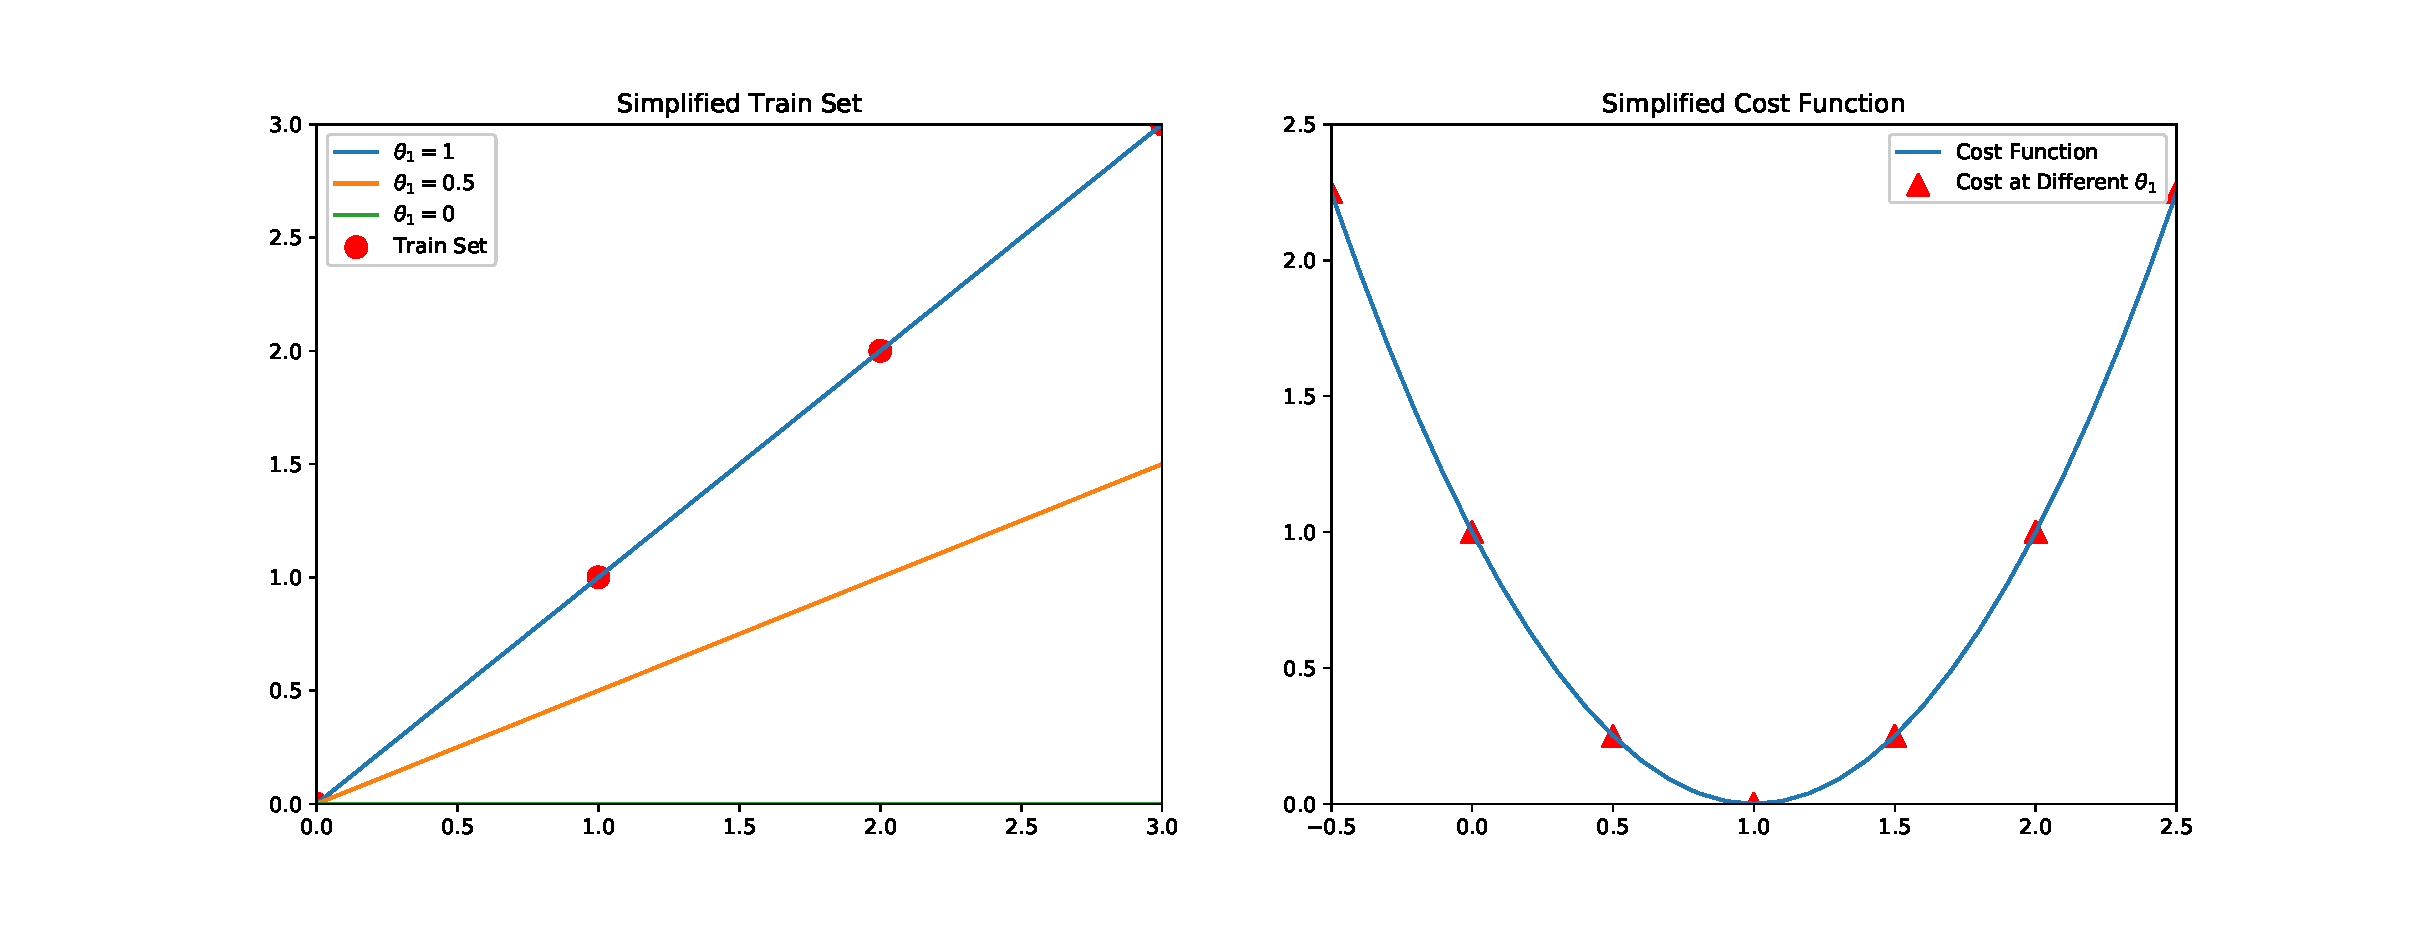
\includegraphics[width=1\textwidth]{OneParameterCostFunction.eps}
\end{figure}

将这些点连在一起形成的曲线,就构成了一个参数下的代价函数曲线。实际上,将三个样本点带入后,可以得到这里的代价函数$J(\theta_1)$的解析式为$J(\theta_1)=\frac{14}{6}(\theta_1-1)^2$。

在课程中,展示了非常漂亮的等高线图及使用梯度下降法找到最优$\theta_0, \theta_1$的图像,但是通过实际测试,并不能画出类似的图像,此处是是否是个人理解出现问题存疑,将代码和对应的图片放在这里作为后续参考:

\begin{lstlisting}[language=Python]
import numpy as np
import matplotlib.pyplot as plt
from mpl_toolkits.mplot3d import Axes3D

x = np.arange(0, 10, 0.05)
y = x + np.random.rand(len(x)) * 2

reg = linear_model.LinearRegression()
reg.fit(x.reshape(-1, 1), y)

theta0 = theta1 = np.linspace(-2.5, 4)
theta0, theta1 = np.meshgrid(theta0, theta1)
err = 0.0
for i in range(len(x)):
    err += np.power((theta0 + theta1 * x[i] - y[i]), 2)
err = err / (2 * len(x))

plt.figure(figsize=(18, 6))
ax1 = plt.subplot(121)
ax1.scatter(x, y)
ax1.plot(x, reg.predict(x.reshape(-1, 1)), color='r')
ax1.set_title('Linear Regression')

ax2 = plt.subplot(122, projection='3d')
ax2.plot_surface(theta0, theta1, err, cmap='rainbow')
ax2.contour(theta0, theta1, err, zdir='r', offset=-2)
ax2.set_title('Cost Function')
           \end{lstlisting}

\begin{figure}[H]
    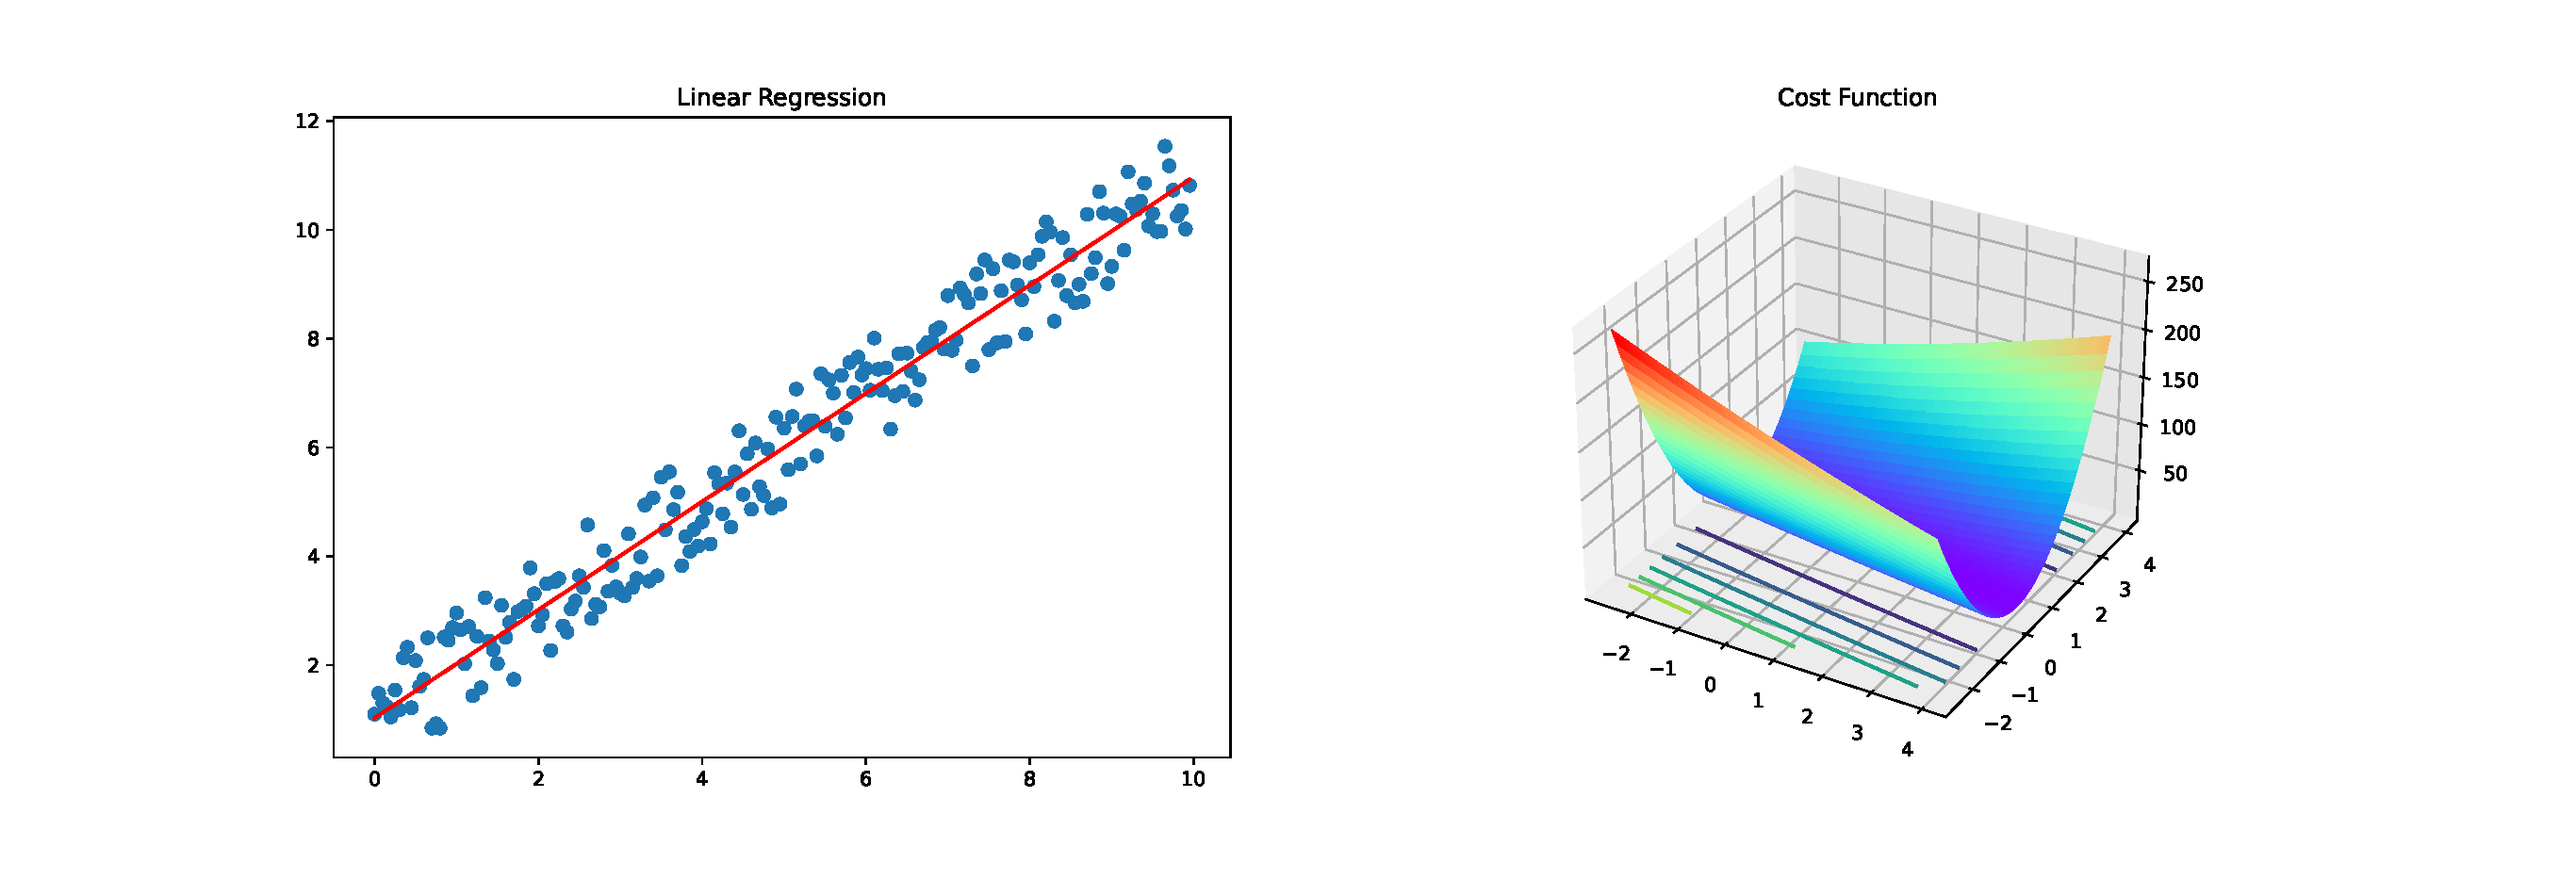
\includegraphics[width=1\textwidth]{CostFunction.eps}
\end{figure}

\subsection{梯度下降}

当有了代价函数$J$之后,就需要找到使代价函数$J$最小的$\theta_0, \theta_1$。梯度下降法就是一种非常好的用来求函数最小值的算法。其本质是每次迭代中找出函数在当前参数下下降最快的方向,然后逐步迭代找到局部最小值。当需要优化的函数是一个凸函数时,局部最小值也是全局最小值。此外,梯度下降要求给出一个学习速率(learning rate)$\alpha$,这对应着每次迭代时所移动的步长。

这里使用的梯度下降算法为批梯度下降(batch gradient descent),即在每次迭代中必须要同时更新所有需要优化的参数,让所有的参数减去学习速率乘以代价函数的导数,然后才能进行下一次迭代。

批量梯度下降算法为:

\begin{equation*}
    \theta_j:=\theta_j-\alpha\frac{\partial}{\partial\theta_j}J(\theta)
\end{equation*}

在梯度下降算法中,学习速率的选择需要一些技巧。如果学习速率选择的过小,则算法收敛至局部最小值所消耗的时间过长,而如果学习速率选择的过大,则可能会导致迭代越过最低点,从而无法找到局部最小值甚至导致算法结果从收敛转向发散。

回到前面两个参数的线性回归问题中,对于线性回归问题使用梯度下降法,关键在于求出代价函数的导数,即:

\begin{align*}
    \frac{\partial}{\partial\theta_j}J(\theta)                                & =\frac{\partial}{\partial\theta_j}\frac{1}{2m}\sum_{i=1}^{n}(h_\theta(x^{(i)})-y^{(i)})^2 \\
    \text{if}\ j=0:\quad\frac{\partial}{\partial\theta_0}J(\theta_0,\theta_1) & =\frac{1}{m}\sum_{i=1}^{m}(h_\theta(x^{(i)})-y^{(i)})                                     \\
                                                                              & =\frac{1}{m}\sum_{i=1}^{m}(\theta_0+\theta_1x_i-y_i)                                      \\
    \text{if}\ j=1:\quad\frac{\partial}{\partial\theta_1}J(\theta_0,\theta_1) & =\frac{1}{m}\sum_{i=1}^{m}((h_\theta(x^{(i)})-y^{(i)})\cdot x^{(i)})                      \\
                                                                              & =\frac{1}{m}\sum_{i=1}^{m}((\theta_0+\theta_1x_i-y_i)\cdot x_i)
\end{align*}

从而:

\begin{align*}
    \theta_0 & :=\theta_0-\alpha\frac{1}{m}\sum_{i=1}^{m}(\theta_0+\theta_1x_i-y_i)            \\
    \theta_1 & :=\theta_1-\alpha\frac{1}{m}\sum_{i=1}^{m}((\theta_0+\theta_1x_i-y_i)\cdot x_i)
\end{align*}

仍然使用之前的示例,尝试进行线性回归并验算结果:

\begin{enumerate}
    \item 
          首先导入必要的Python库并构造数据集:
          
          \begin{lstlisting}[language=Python]
import numpy as np
# 指定使用的随机数种子
np.random.seed(0)

# 创建模拟数据
x = np.arange(0, 10, 0.05)
y = x + np.random.rand(len(x)) * 2
               \end{lstlisting}
          
    \item 
          进行梯度下降算法:
          
          使用矩阵计算代价函数对于参数$\theta$的偏导:
          
          \begin{align*}
              \theta_j & :=\theta_j-\alpha\frac{\partial}{\partial\theta_j}J(\theta)                                         \\
              \theta_j & :=\theta_j-\alpha\frac{\partial}{\partial\theta_j}(\frac{1}{2m}\sum_{i=1}^{m}(h_\theta(x^i)-y^i))^2 \\
              \theta_j & :=\theta_j-\frac{\alpha}{m}\sum_{i=1}^{m}(\theta_0x_0^i+\theta_1x_1^i+\dots-y^i)\cdot x_j^i
          \end{align*}
          
          对于一个$(m\times j)$的矩阵$X$,$m$为样本数量,$j$为特征$x$的数量,有对应的系数为$(1\times j)$的矩阵$\Theta$及$(m\times 1)$的因变量矩阵$Y$,可以将代价函数的导数部分化简为:
          
          \begin{align*}
              X \times \Theta^T & = 
              \left[
                  \begin{matrix}
                      x_0^1  & x_1^1  & \cdots & x_j^1  \\
                      x_0^2  & x_1^2  & \cdots & x_j^2  \\
                      \vdots & \vdots & \ddots & \vdots \\
                      x_0^m  & x_1^m  & \cdots & x_j^m
                  \end{matrix}
                  \right]
              \left[
                  \begin{matrix}
                      \theta_0 \\
                      \theta_1 \\
                      \cdots   \\
                      \theta_j  
                  \end{matrix}
                  \right]            \\
                                & = 
              \left[
                  \begin{matrix}
                      \theta_0x_0^1+\theta_1x_1^1+\dots+\theta_jx_j^1 \\
                      \vdots                                          \\
                      \theta_0x_0^m+\theta_1x_1^m+\dots+\theta_jx_j^m \\
                  \end{matrix}
                  \right]
          \end{align*}
          
          因此:
          
          \begin{align*}
                & \left[
                  \begin{matrix}
                       & \sum_{i=1}^{m}(\theta_0x_0^i+\theta_1x_1^i+\dots+\theta_jx_j^i-y^i)\cdot x_0^i \\
                       & \vdots                                                                         \\
                       & \sum_{i=1}^{m}(\theta_0x_0^i+\theta_1x_1^i+\dots+\theta_jx_j^i-y^i)\cdot x_j^i \\
                  \end{matrix}
                  \right] \\
              = & 
              \left[
                  \begin{matrix}
                      x_0^1  & \cdots & x_0^m  \\
                      \vdots & \ddots & \vdots \\
                      x_j^1  & \cdots & x_j^m
                  \end{matrix}
                  \right]
              \left(\left[
                  \begin{matrix}
                      \theta_0x_0^1+\theta_1x_1^1+\dots+\theta_jx_j^1 \\
                      \vdots                                          \\
                      \theta_0x_0^m+\theta_1x_1^m+\dots+\theta_jx_j^m \\
                  \end{matrix}
                  \right]-
              \left[
                  \begin{matrix}
                      y^1    \\
                      \vdots \\
                      y^m
                  \end{matrix}
                  \right]\right)
          \end{align*}
          
          即:
          
          \begin{align*}
              \theta_j          & :=\theta_j-\frac{\alpha}{m}\sum_{i=1}^{m}(\theta_0x_0^i+\theta_1x_1^i+\dots-y^i)\cdot x_j^i \\
              \Rightarrow\Theta & :=\Theta-\frac{\alpha}{m}X^T(X\times \Theta^T-Y)
          \end{align*}
          
          当只有两个参数$\theta_0,\theta_1$时,由于$\theta_0$对应的是截距项,因此可以对$x$增加全为1的列作为$x_0$,使其可以进行矩阵运算,同时设定学习速率$\alpha$和初始点:
          
          \begin{lstlisting}[language=Python]
X = np.stack((np.ones(len(x)), x), axis=1)
Y = y
# 设定学习速率
alpha = 0.01
# 设定初始点
theta = np.array([0.0, 0.0])
gradient = alpha / len(y) * (X.T.dot(X.dot(theta.T) - Y))
# 计算代价函数
cost = np.sum(np.power(X.dot(theta.T) - Y, 2)) / (2 * len(y))
costs = [cost]
while not (np.isclose(gradient[0], 0) and np.isclose(gradient[1], 0)):
    theta = theta - gradient
    gradient = alpha / len(y) * (X.T.dot(X.dot(theta.T) - Y))
    cost = np.sum(np.power(X.dot(theta.T) - Y, 2)) / (2 * len(y))
    costs.append(cost)
print("Iteration: {}, theta_0={:.4f}, theta_1={:.4f}".format(len(costs), theta[0], theta[1]))
# Iteration: 4974, theta_0=1.0283, theta_1=0.9945
               \end{lstlisting}
          
          在迭代4974次后$\theta$变化量约等于0,迭代结束,得到计算出的$\theta$值。
          
    \item 
          使用scikit-learn进行线性回归,校验梯度下降得出的结果:
          
          \begin{lstlisting}[language=Python]
from sklearn import linear_model
reg = linear_model.LinearRegression()
reg.fit(x.reshape(-1, 1), y)
print("theta_0={:.4f}, theta_1={:.4f}".format(reg.intercept_, reg.coef_[0])))
# theta_0=1.0283, theta_1=0.9945
               \end{lstlisting}
          
          结果一致。
\end{enumerate}

\section{线性代数回顾 Linear Algebra Review}

\begin{enumerate}
    \item 
          矩阵乘法不服从交换律:$A\times B\neq B\times A$。
    \item 
          矩阵乘法服从结合律:$A\times(B\times C) = (A\times B)\times C$。
    \item 
          单位矩阵$I$类似于数乘中的1,$I$是一个方阵,满足$AA^{-1}=A^{-1}A=I$。对于任意矩阵,$AI=IA=A$,这里两个单位矩阵的维度不一定是相同的,其维度隐含在$A$的维度中。
    \item 
          只有方阵才有逆矩阵,但不是所有方阵都有逆矩阵。没有逆矩阵的矩阵称为奇异矩阵。
    \item 
          矩阵转置的基本性质:
          
          \begin{align*}
               & (A\pm B)^T = A^T\pm B^T       \\
               & (A\times B)^T = B^T\times A^T \\
               & (A^T)^T = A                   \\
               & (KA)^T = KA^T
          \end{align*}
\end{enumerate}

\section{多元线性回归 Linear Regression with Multiple Variables}

在单变量线性回归中,

\begin{equation*}
    h_\theta(x) = \theta_0 + \theta_1x_1
\end{equation*}

在多元线性回归中,$h_\theta(x)$将拓展为:

\begin{equation*}
    h_\theta(x)=\theta_0 + \theta_1x_1+ \theta_2x_2+\cdots+\theta_nx_n
\end{equation*}

同样,为了便于使用矩阵形式表述,定义$x_0=1$,因此,

\begin{equation*}
    h_\theta(x)=\theta_0x_0 + \theta_1x_1+ \theta_2x_2+\cdots+\theta_nx_n
\end{equation*}

在这里:

\begin{equation*}
    X=\left[
        \begin{matrix}
            x_0    \\
            x_1    \\
            \vdots \\
            x_n
        \end{matrix}
        \right]\in\mathbb{R}^{n+1}\quad
    \Theta=\left[
        \begin{matrix}
            \theta_0 \\
            \theta_1 \\
            \vdots   \\
            \theta_n
        \end{matrix}
        \right]\in\mathbb{R}^{n+1}
\end{equation*}

从而有:

\begin{align*}
    h_\theta(x) & =\theta_0x_0 + \theta_1x_1+ \theta_2x_2+\cdots+\theta_nx_n \\
                & =\Theta^TX
\end{align*}

和单变量线性回归一样,这里给出多元线性回归的模型表示:

\begin{align*}
     & \mathbf{Hypothesis}: h_\theta(x)=\Theta^TX=\theta_0x_0 + \theta_1x_1 + \theta_2x_2+\cdots+\theta_nx_n                          \\
     & \mathbf{Parameters}:\Theta=\theta_0,\theta_1,\dots,\theta_n                                                                    \\
     & \mathbf{Cost Function}:J(\Theta)=J(\theta_0,\theta_1,\dots,\theta_n) = \frac{1}{2m}\sum_{i=1}^{m}(h_\theta(x^{(i)})-y^{(i)})^2 \\
     & \mathbf{Goal}: \mathop{minimize}\limits_{\Theta}J(\Theta)
\end{align*}

批量梯度下降算法同样为(注意对每个$j=0,\dots,n$要同步更新$\theta$):

\begin{equation*}
    \theta_j:=\theta_j-\alpha\frac{\partial}{\partial\theta_j}J(\Theta)
\end{equation*}


\subsection{特征缩放}

在面对多维特征问题时,最好需要保证这些特征具有相近的尺度,从而帮助梯度下降算法更快的收敛。在课程的房价问题中,如果使用房屋尺寸和数量两个特征,显然房屋尺寸的值会比房屋数量大很多,在等高线图上会表现为扁而狭长的图像,这会使得梯度下降算法需要非常多次的迭代才能收敛到全局最小值。

这种问题的解决方法是尝试将所有特征的尺度都尽量缩放到-1和1之间,最常用的方法是令$x_n=\frac{x_n-\mu_n}{s_n}$,其中$\mu_n$是均值,$s_n$是标准差。

\subsection{学习速率}

通过画出迭代次数与代价函数的关系图表,可以直观看出算法在何处收敛。正确运行的梯度下降算法应当在每次迭代后都降低代价函数。

可以证明出,当学习速率$\alpha$足够小的时候,代价函数一定会在每次迭代时都降低,因此如果出现异常,在排除代码错误后通常应当选择更小的学习速率。但是过小的学习速率会导致需要大量迭代才会收敛到结果,因此选择学习速率需要进行一定的权衡。

\subsection{特征和多项式回归}

当线性回归并不适用于数据时,选择一个多项式进行拟合也是合适的方法。通过将特征进行变换,例如三次模型:$h_\theta(x)=\theta_0+\theta_1x_1+\theta_2x_1^2+\theta_3x_1^3$中,可以设置令$x_2=x_1^2,x_3=x_1^3$从而将多项式转换为线性回归。但是这种方式如果需要使用梯度下降算法,尽量进行特征缩放,以避免特征的取值范围差距过大。

\subsection{正规方程}

除了使用梯度下降进行迭代的算法以外,同样可以有解析的方式一次性解出$\Theta$而不需要反复迭代。

在一个标准的线性回归问题中,对于$\Theta\in\mathbb{R}^{n+1}$,需要最小化代价函数$J(\theta_0,\theta_1,\dots,\theta_n)=\frac{1}{2m}\sum_{i=1}^{m}(h_\theta(x^{(i)})-y^{(i)})^2$时,微积分的方式是对$J(\Theta)$中的每个参数求偏导,并令所有参数的偏导数为0时得到$\Theta$的值,即对每个$\theta$,$\frac{\partial}{\partial\theta_j}J(\Theta)=0$。

最终可以解出向量$\Theta=(X^TX)^{-1}X^Ty$。以下是推导过程:

\textbf{Note}:约定$X=(x_1, x_2,\dots,x_N)^T$
\begin{align*}
    \frac{\partial a}{\partial X}     & = 0                           \\
    \frac{\partial X}{\partial X}     & = I                           \\
    \frac{\partial AX}{\partial X}    & = A^T                         \\
    \frac{\partial X^TA}{\partial X}  & = A                           \\
    \frac{\partial X^TAX}{\partial X} & = (A+A^T)X                    \\
    \frac{\partial X^TAX}{\partial X} & = 2AX \text{(A is symmetric)}
\end{align*}

因此:
\begin{align*}
    J(\Theta) & = \frac{1}{2m}\sum_{i=1}^{m}(h_\theta(x^{(i)})-y^{(i)})^2       \\
              & = \frac{1}{2m}(X\Theta-y)^2                                     \\
              & = \frac{1}{2m}(X\Theta-y)^T(X\Theta-y)                          \\
              & = \frac{1}{2m}(\Theta^TX^T-y^T)(X\Theta-y)                      \\
              & = \frac{1}{2m}(\Theta^TX^TX\Theta-\Theta^TX^Ty-y^TX\Theta+y^Ty)
\end{align*}

代价函数对$\Theta$求偏导并等于0:
\begin{align*}
    \frac{\partial J(\Theta)}{\partial\Theta} & = \frac{1}{2m}(2X^TX\Theta-X^Ty-X^Ty+0) \\
                                              & = \frac{1}{2m}(2X^TX\Theta-2X^Ty) = 0   \\
                                              & \Rightarrow X^TX\Theta-X^Ty=0           \\
\end{align*}

从而可以得出$\Theta=(X^TX)^{(-1)}X^Ty$

这种方法对于奇异矩阵无效,因为无法计算矩阵的逆。在Numpy中,可以使用数值算法计算广义逆矩阵。

\begin{lstlisting}[language=Python]
    import numpy as np
    # 非奇异矩阵
    inv = np.linalg.inv(np.array)
    # 对于Matrix对象
    # inv = np.matrix.I
    # 奇异矩阵求伪逆(广义逆矩阵)
    inv = np.linalg.pinv(np.array)
\end{lstlisting}

显然,在正规方程计算中可以不需要使用特征缩放。

正规方程方法在特征值较少的情况下可以通过一次运算得出,效率较高,但是当特征数量较多时,由于计算逆矩阵的时间复杂度为$O(n^3)$,因此当有超过10000个特征时,使用正规方程方法就较为不合适。同时,正规方程法只适用于线性模型而对其他模型无效,梯度下降法的适用范围更广。‘

\section{逻辑回归 Logistic Regression}

\subsection{分类问题}

在分类问题中,预测的变量$y$是离散值。在最基础的二元分类问题中,因变量$y$只有两个结果,分别称为负向类(negative class)和正向类(positive class),即因变量$y\in\{0, 1\}$。假定阈值设置为0.5,如果预测值超过阈值则判定为正向,否则判定为负向。

如果使用线性回归对其进行预测,会出现两个显著的问题:

\begin{enumerate}
    \item 分类问题只有两个可能,0或1,但线性回归得到的输出值可能远大于1或远小于0,即使训练样本的$y$都等于0或1。
    \item 如果训练集中有离群点,会扭曲回归的假设函数,使之前设定的阈值(例如0.5)显得不再合适,从而导致预测能力下降。
\end{enumerate}

因此,对于分类问题使用新的算法:逻辑回归。逻辑回归尽管名称中带有“回归”二字,但是却是一个分类算法。逻辑回归可以保证输出值永远在0到1之间。

给出分类问题的定义:

\begin{itemize}
    \item Classification: $y\in\{0, 1\}$
    \item Want: $0\leq h_\theta(x)\leq 1$
    \item Hypothesis: $h_\theta(x)=g(\theta^Tx)$
    \item Sigmoid Function: $g(z)=\frac{1}{1+e^{-z}}$
\end{itemize}

即:

\begin{equation*}
    h_\theta(x)=\frac{1}{1+e^{-\theta^Tx}}
\end{equation*}

$h_\theta(x)$表示,在给定输入$x$时,预测$y=1$的概率,也相当于$h_\theta(x)=\mathbb{P}(y=1|x; \theta)$。

\subsection{决策边界}

在逻辑回归中,设定阈值0.5,预测当$h_\theta(x)\geq 0.5$时,$y=1$,否则$y=0$。

根据逻辑回归中的函数$g(z)=\frac{1}{1+e^{-z}}$图像,可以知道当$z>0$时$g(z)>0.5$,否则$g(z)<0.5$,又因为$z=\theta^Tx$,即$\theta^Tx\geq 0$时,预测$y=1$,否则预测$y=0$。在这里,$z$对应的就是决策边界。

假定一个模型:
\begin{equation*}
    h_\theta(x)=g(\theta_0+\theta_1x_1+\theta_2x_2)
\end{equation*}

已知参数:

\begin{equation*}
    \theta=\left[
        \begin{matrix}
            -3 \\
            1  \\
            1
        \end{matrix}
        \right]
\end{equation*}

则当$x_1+x_2\geq 3$时,模型预测$y=1$,这里,$x_1+x_2\geq 3$形成的分界线就是这个模型的决策边界,将预测为1和预测为0的区域进行了分隔。

\begin{figure}[H]
    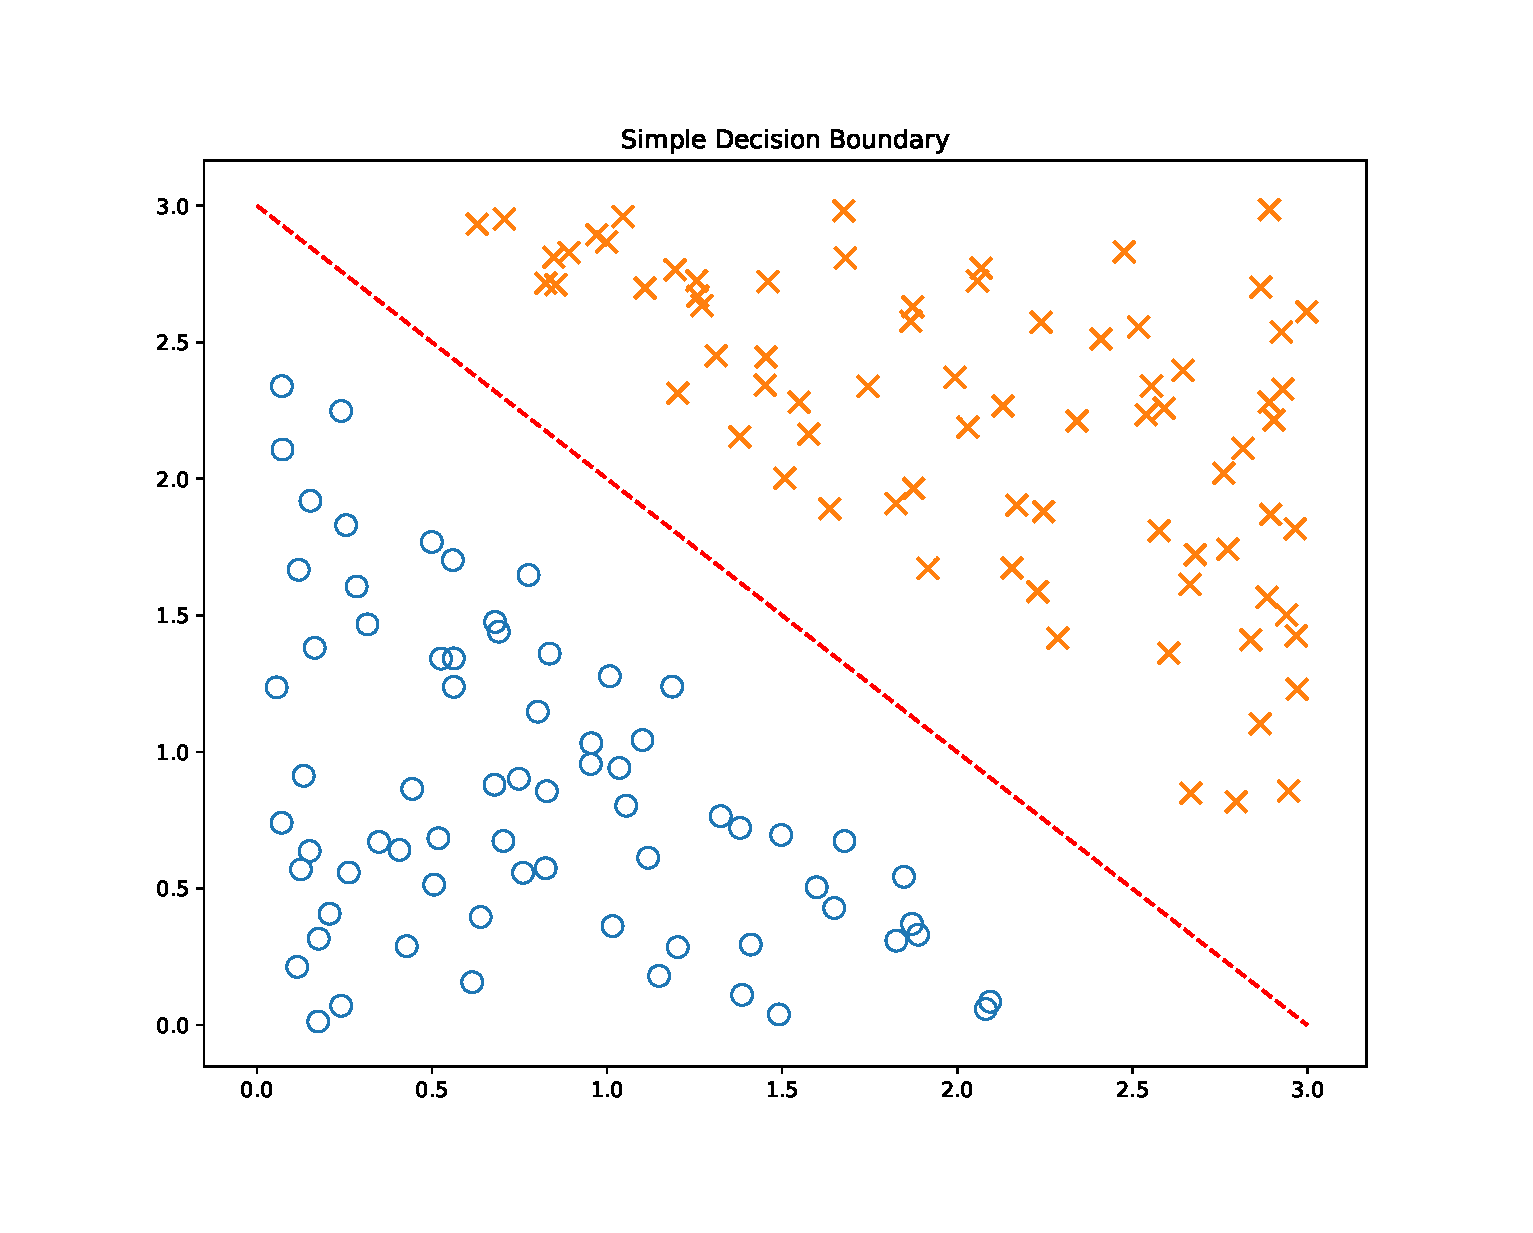
\includegraphics[width=1\textwidth]{SimpleDecisionBoundary.eps}
\end{figure}

决策边界同样可以是非线性的,例如模型

\begin{equation*}
    h_\theta(x)=g(\theta_0+\theta_1x_1+\theta_2x_2+\theta_3x_1^2+\theta_4x_2^2)
\end{equation*}

其对应的参数

\begin{equation*}
    \theta=\left[
        \begin{matrix}
            -1 \\
            0  \\
            0  \\
            1  \\
            1
        \end{matrix}
        \right]
\end{equation*}

可以得到决策边界为一个圆心为原点,半径为1的圆:$x_1^2+x_2^2=1$。

\begin{figure}[H]
    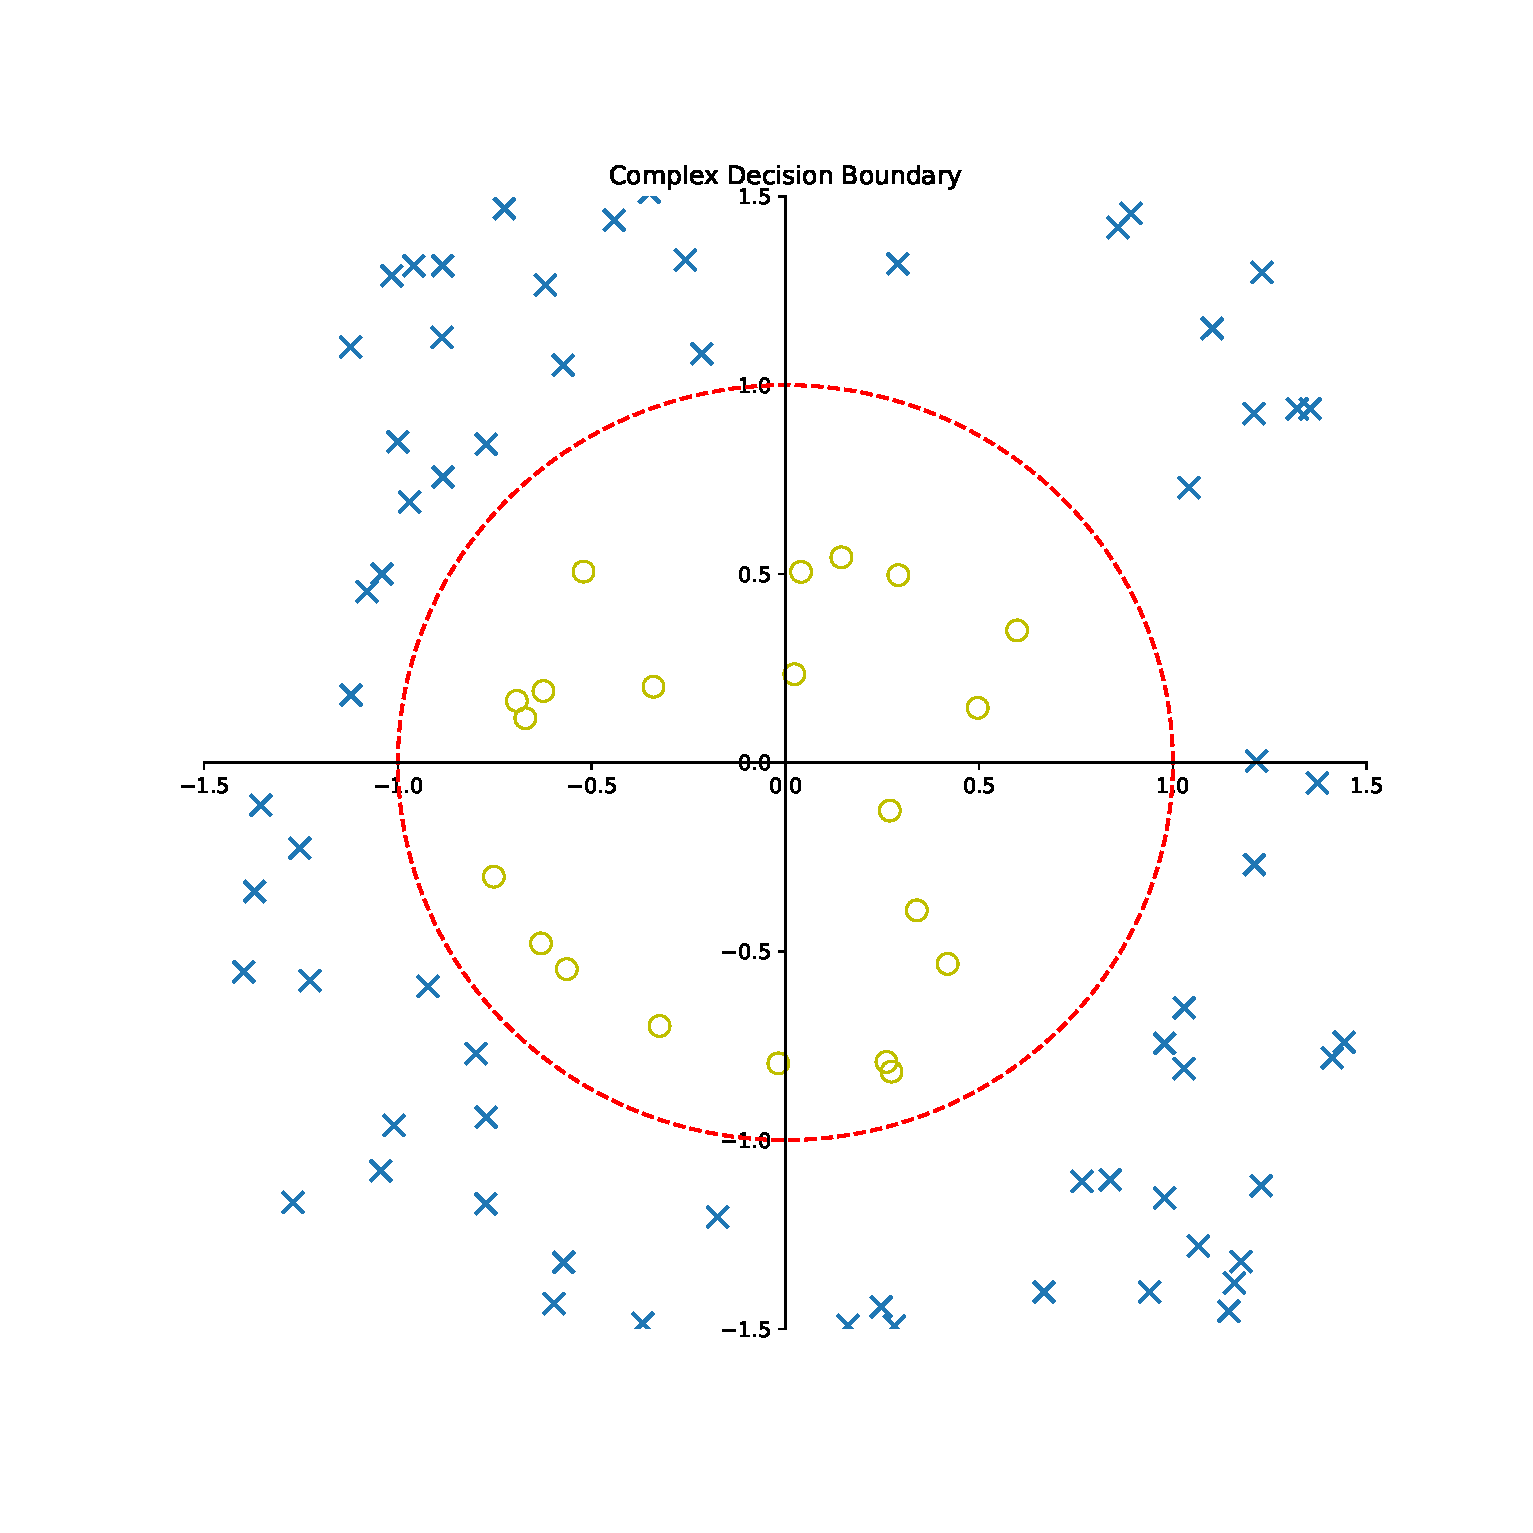
\includegraphics[width=1\textwidth]{ComplexDecisionBoundary.eps}
\end{figure}

决策边界可以非常复杂,可以用复杂的模型$z$来适应复杂的决策边界。

\subsection{代价函数}

对于逻辑回归,同样需要定义一个代价函数用于拟合模型的参数$\theta$。

\begin{align*}
     & \mathbf{Training\ set}: \{(x^{(1)}, y^{(1)}), (x^{(2)}, y^{(2)}), \dots, (x^{(m)}, y^{m})\} \\
     & \mathbf{Hypothesis}: h_\theta(x)=\frac{1}{1+e^{-\theta^Tx}}                                 \\
     & \mathbf{Given\ examples}: x\in\left[
        \begin{matrix}
            x_0   \\
            x_1   \\
            \dots \\
            x_n
        \end{matrix}
        \right] x_0=1, y\in\{0, 1\}
\end{align*}

对于线性回归模型,定义的代价函数是模型误差的平方和:

\begin{align*}
    J(\theta) & = \frac{1}{2m}\sum_{i=1}^{m}(h_\theta(x^{(i)})-y^{(i)})^2 \\
              & = \mathtt{Cost}(h_\theta(x^{(i)}, y))
\end{align*}

理论来说,逻辑回归同样可以使用类似的代价函数。但是,如果将$h_\theta(x)=\frac{1}{1+e^{-\theta^Tx}}$代入这个代价函数中时,代价函数会是一个非凸函数(non-convex function)。这意味着代价函数会有许多局部最小值,从而影响梯度下降算法寻找全局最小值。

因此,在逻辑回归中,定义新的代价函数为:

\begin{equation*}
    \mathtt{Cost}(h_\theta(x), y) = 
    \begin{cases}
        -\log(h_\theta(x)),   & y = 1 \\
        -\log(1-h_\theta(x)), & y = 0
    \end{cases}
\end{equation*}

这样构建的代价函数有良好的性质,当实际$y=1$且$h_\theta(x)=1$时,误差为0,当$y=1$但$h_\theta(x)$不为1时,误差随$h_\theta(x)$变小而变大,并趋向于正无穷$\infty$,相反时也是一样。

以上函数可以简化为如下更为紧凑的形式:

\begin{equation*}
    \mathtt{Cost}(h_{\theta}(x), y) = -y\log(h_\theta(x)) - (1-y)\log(1-h_\theta(x))
\end{equation*}

因此,代价函数最后为:

\begin{align*}
    J(\theta) & = \frac{1}{m}\sum^{m}_{i=1}\mathtt{Cost}(h_\theta(x^{(i)}), y^{(i)})                                 \\
              & = -\frac{1}{m}[\sum^{m}_{i=1}y^{(i)}\log h_\theta(x^{(i)}) + (1 - y^{(i)})\log(1-h_\theta(x^{(i)}))]
\end{align*}

找到参数$\theta$即最小化代价函数$J(\theta)$。

同样找到参数$\theta$的方式是使用梯度下降算法:

\begin{equation*}
    \theta_j:=\theta_j-\alpha\frac{\partial}{\partial\theta_j}J(\theta)
\end{equation*}

同样要对每个$j=0,\dots,n$同步更新$\theta$。

要计算$\frac{\partial}{\partial\theta_j}J(\theta)$,需要使用复合函数求导的链式法则:

\begin{equation*}
    \frac{d}{dx}g(f(x)) = g'(f(x))f'(x)
\end{equation*}

或者写作

\begin{equation*}
    \frac{du}{dx} = \frac{du}{dy}\cdot\frac{dy}{dx}
\end{equation*}

同时,$h_\theta(x^i) = g(\theta^Tx)$,sigmoid函数$g(z) = \frac{1}{1+e^{-z}}$的导数为:

\begin{align*}
    \frac{d}{dz}g(z) & = \frac{d}{dz}\frac{1}{1+e^{-z}} \\
    & = -\frac{-e^{-z}}{(1+e^{-z})^2}\\
    & = \frac{e^{-z}}{(1+e^{-z})^2} \\
    & = \frac{1}{1+e^{-z}}\frac{e^{-z}}{1+e^{-z}}\\
    & = g(z)(1-g(z))
\end{align*}

根据以上可以得出

\begin{align*}
    \frac{\partial}{\partial\theta_j}J(\theta) =&-\frac{1}{m}\sum_{i=1}^{m}\frac{\partial}{\partial\theta_j}(y^{(i)}\log h_\theta(x^{(i)})+(1-y^{(i)})\log(1-h_\theta(x^{(i)})))\\
     =&-\frac{1}{m}\sum_{i=1}^{m}\frac{\partial}{\partial\theta_j}(y^{(i)}\log g(\theta^Tx)+(1-y^{(i)})\log(1-g(\theta^Tx)))\\
     =&-\frac{1}{m}\sum_{i=1}^{m}(\frac{\partial}{\partial\theta_j}y^{(i)}\log g(\theta^Tx) + \frac{\partial}{\partial\theta_j}(1-y^{(i)})\log(1-g(\theta^Tx))) \\
     =&-\frac{1}{m}\sum_{i=1}^{m}(y^{(i)}\frac{\partial}{\partial g(\theta^Tx)}\log g(\theta^Tx)\cdot\frac{\partial}{\partial\theta^Tx}g(\theta^Tx)\cdot\frac{\partial}{\partial\theta_j}\theta^Tx\\
     &+(1-y^{(i)})\frac{\partial}{\partial g(\theta^Tx)}\log(1-g(\theta^Tx))\cdot\frac{\partial}{\partial\theta^Tx}g(\theta^Tx)\cdot\frac{\partial}{\partial\theta_j}\theta^Tx) \\
     =&-\frac{1}{m}\sum_{i=1}^{m}(y^{(i)}\frac{1}{g(\theta^Tx)}\cdot g(\theta^Tx)(1-g(\theta^Tx))\cdot x_j \\
     &+(1-y^{(i)})\frac{-1}{1-g(\theta^Tx)}\cdot g(\theta^Tx)(1-g(\theta^Tx))\cdot x_j) \\
     =&-\frac{1}{m}\sum_{i=1}^{m}(y^{(i)}-g(\theta^Tx))x_j \\
     =&\frac{1}{m}\sum_{i=1}^{m}(h_\theta(x^{(i)})-y^{(i)})x_j
\end{align*}

因此,

\begin{equation*}
    \theta_j:=\theta_j-\alpha\sum_{i=1}^{m}(h_\theta(x^{(i)})-y^{(i)})x_j^{(i)}
\end{equation*}

显然,这个梯度下降算法和线性回归时使用的梯度下降算法公式完全相同,但是由于$h_\theta(x)$在这里的值为$\frac{1}{1+e^{-\theta^Tx}}$而在线性回归中$h_\theta(x)$为$\theta^Tx$,因此,尽管更新$\theta$的方法相同,但是这两个梯度下降算法并不相同。

\subsection{高级优化与多元分类}

除了梯度下降算法之外,还有很多其他高级优化方法可以使用,例如共轭梯度法(Conjugate gradient),变尺度法(BFGS),限制变尺度法(L-BFGS)等。这些方法通常有更快的收敛速度,对于更大的特征也有更好的表现,同时有些(例如这三种)不需要手动选择学习速率$\alpha$,但是这些算法也意味着更加复杂,更加难以调试。

当$y$有超过两个分类(0/1)时,就构成一个多分类问题。为了解决这种问题,可以将其中一类作为正向类1,其余所有分类作为负向类0,随后将另一个分类作为正向类1,其余所有分类作为负向类0并以此类推,直到得到一系列的模型:

\begin{equation*}
    h_\theta^{(i)}(x) = \mathbb{P}(y=i|x; \theta), i=(1,2,3,\dots,k)
\end{equation*}

当需要做出预测时,将所有的分类机运行一遍,对每个分类输入变量,然后选择最高可能性的输出变量,即$\mathop{max}\limits_ih_\theta^{(i)}(x)$。

\section{正则化 Regularization}

\section{神经网络:表述 Neural Networks: Representation}

\section{神经网络:学习 Neural Networks: Learning}

\section{应用机器学习的建议 Advice for Apply Machine Learning}

\section{机器学习系统的设计 Machine Learning System Design}

\section{支持向量机 Support Vector Machines}

\section{聚类 Clustering}

\section{降维 Dimensionality Reduction}

\section{异常检测 Anomaly Detection}

\section{推荐系统 Recommender Systems}

\section{大规模机器学习 Large Scale Machine Learning}

\section{结语 Conclusion}

\end{document}